\documentclass[conference]{inc/IEEEtran}
\IEEEoverridecommandlockouts
% The preceding line is only needed to identify funding in the first footnote. If that is unneeded, please comment it out.
% !TeX root = ../main.tex
\usepackage{a4wide}

\usepackage[utf8]{inputenc}

%\usepackage[ngerman]{babel}
\usepackage[english]{babel}

\usepackage[T1]{fontenc}
\usepackage{palatino}
\usepackage{cite}
\usepackage{graphicx}
\usepackage{caption}
\usepackage{url}
\usepackage{acronym}
\usepackage{tocloft}
\usepackage{algorithmic}
\usepackage{mathpazo}
\usepackage{amsmath}
\usepackage{amsfonts}
\usepackage{adjustbox}
\usepackage{textcomp}
%\usepackage{subcaption}

\usepackage{hhline}
\usepackage{fancyhdr}
\usepackage{amssymb}
\usepackage{floatflt}
\usepackage{setspace}
\usepackage{float}
\usepackage{booktabs}
\usepackage{color}
\usepackage{listings}
\usepackage{array}
\usepackage{scrhack}
\usepackage{xcolor}
\usepackage{wrapfig}
\usepackage[hidelinks]{hyperref}
\usepackage{url}
\usepackage{lmodern}
\usepackage{multirow}
\usepackage{subfig}
\usepackage{cleveref}
\usepackage{lipsum}
\usepackage[bottom, hang]{footmisc}


\def\BibTeX{{\rm B\kern-.05em{\sc i\kern-.025em b}\kern-.08em
    T\kern-.1667em\lower.7ex\hbox{E}\kern-.125emX}}
\begin{document}

\title{Neural Network-Based Iris Classification and Genetic Algorithm-Driven SHUBERT Function Optimisation \\
{\footnotesize Completed as part of \textit{M25352 Neural Networks and Genetic Algorithms}}
}


\author{\IEEEauthorblockN{Connor Brook}
    \IEEEauthorblockA{\textit{BSc. Data Science and Analytics} \\
        \textit{University of Portsmouth}\\
        Portsmouth, United Kingdom \\
        brook@connordata.science}
    \and
    \IEEEauthorblockN{Jamie Doe}
    \IEEEauthorblockA{\textit{BSc. Software Engineering} \\
        \textit{University of Portsmouth}\\
        Portsmouth, United Kingdom \\
        UP953068@myport.ac.uk}
}

\maketitle

\begin{abstract}
    In this paper, we explore two different optimisation problems: a neural network for the Iris dataset and a genetic algorithm for the SHUBERT function. We design, implement, and evaluate both optimisation techniques, comparing their performance and discussing the advantages and disadvantages of each method. The artificial neural network is employed to classify iris flowers based on their morphological features, while the genetic algorithm is utilized to optimize the SHUBERT function, a well-known benchmark problem in the global optimisation domain. By comparing the results of these two distinct optimisation approaches, we provide insights into their applicability and effectiveness in solving different types of problems.
\end{abstract}

\section{Introduction}

Optimisation techniques like artificial neural networks (ANNs) and genetic algorithms (GAs) have become prevalent due to their broad applications, including machine learning and finance. This paper applies ANNs for Iris dataset classification and GAs for SHUBERT function optimisation, both complex problems in their respective fields. The comparison of these methods aims to elucidate their strengths, weaknesses, and suitability for different problem types, encompassing their design, implementation, and evaluation.

\section{Part I: Neural Networks for Classification/Mapping Task}

\subsection{Introduction}

The Iris dataset is a classic machine learning classification problem. This report aims to create an artificial neural
network to accurately classify Iris plants into three species: Setosa, Versicolour, and Virginica. We tackle the
challenge of non-linear separability between two species through data preprocessing, neural network design, optimization, 
validation, and evaluation. Our goal is to provide insights and pave the way for future research in this field.

\subsection{Data Analysis and Pre-processing}

\subsubsection{Data Analysis}
First, we need to analyze the Iris dataset using visualization techniques, enabling us to understand the relationships between attributes and the distribution of Iris species before theorizing the ANN's architecture.

\textbf{Boxplot}: We created a boxplot to visualize the distribution of each attribute (sepal length, sepal width,
  petal length, and petal width).

  \begin{figure}
    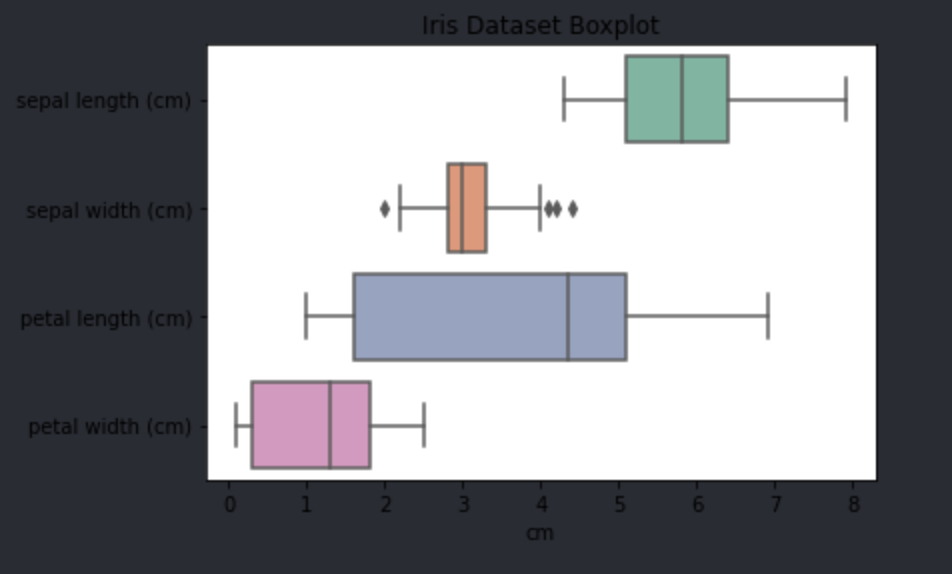
\includegraphics[width=\linewidth]{figures/boxplot.png}
    \caption{Boxplot}
    \label{fig:boat1}
  \end{figure}

\textbf{Pairplot}: A pairplot was generated to illustrate the relationships between all the possible pairs of attributes.
  This scatterplot matrix allowed us to observe the linear separability of Iris Setosa and the evident overlap between
  Iris Versicolour and Iris Virginica.

  \begin{figure}
    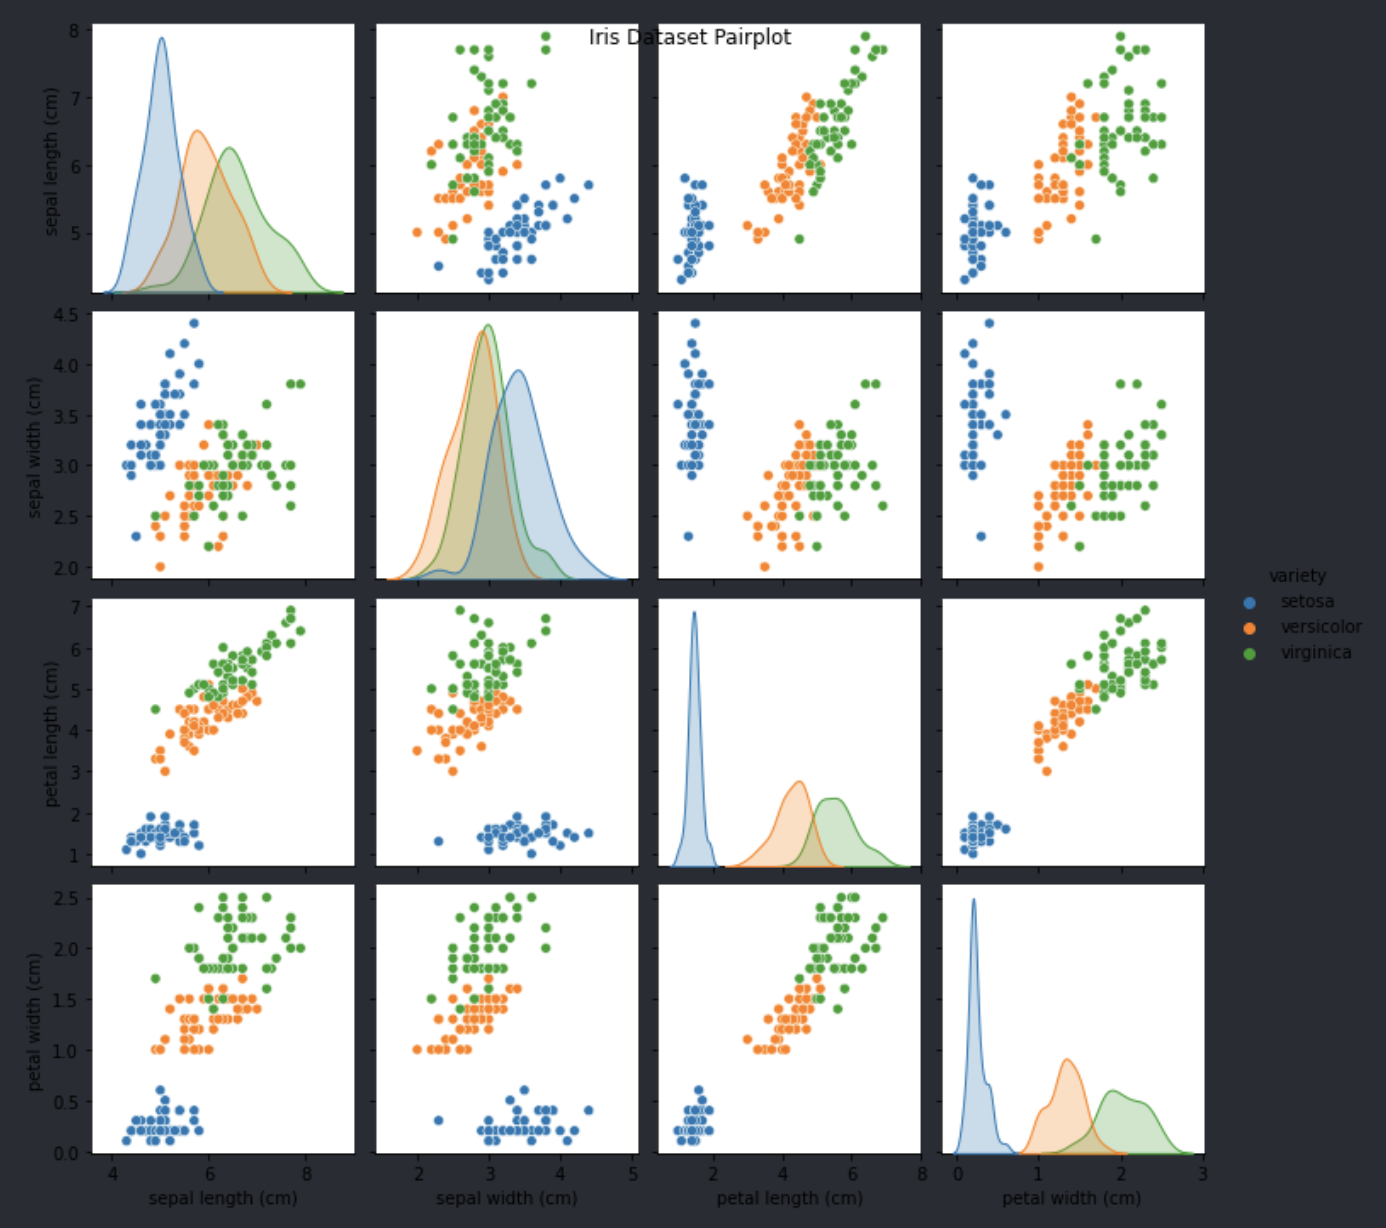
\includegraphics[width=\linewidth]{figures/pairplot.png}
    \caption{Pairplot}
    \label{fig:boat1}
  \end{figure}

\textbf{Correlation Matrix}: We calculated the correlation matrix to quantify the linear relationships between the attributes.
  By using a heatmap, we could easily identify strong positive correlations between petal length and petal width, as well as
  between petal length and sepal length.

  \begin{figure}
    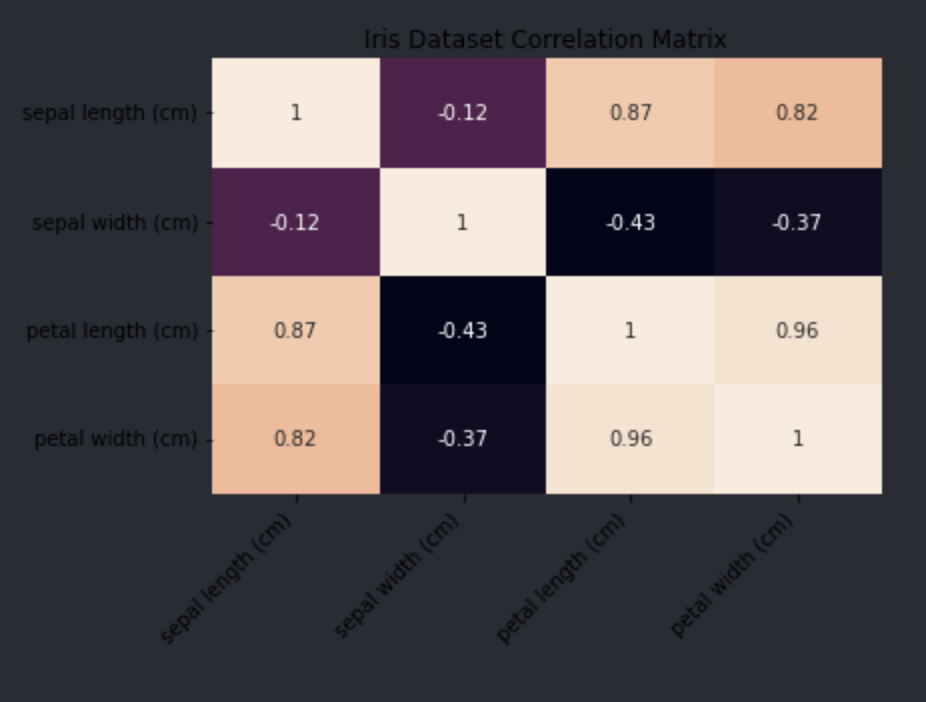
\includegraphics[width=\linewidth]{figures/correlationmatrix.png}
    \caption{Correlation Matrix}
    \label{fig:boat1}
  \end{figure}

\textbf{Principal Component Analysis (PCA)}: We performed PCA with three components to reduce the dimensionality of the dataset
  and project the data onto a lower-dimensional space. A 3D scatterplot was created to visualize the clustering of the Iris
  species in this reduced space, providing insights into the separability of the classes.

  \begin{figure}
    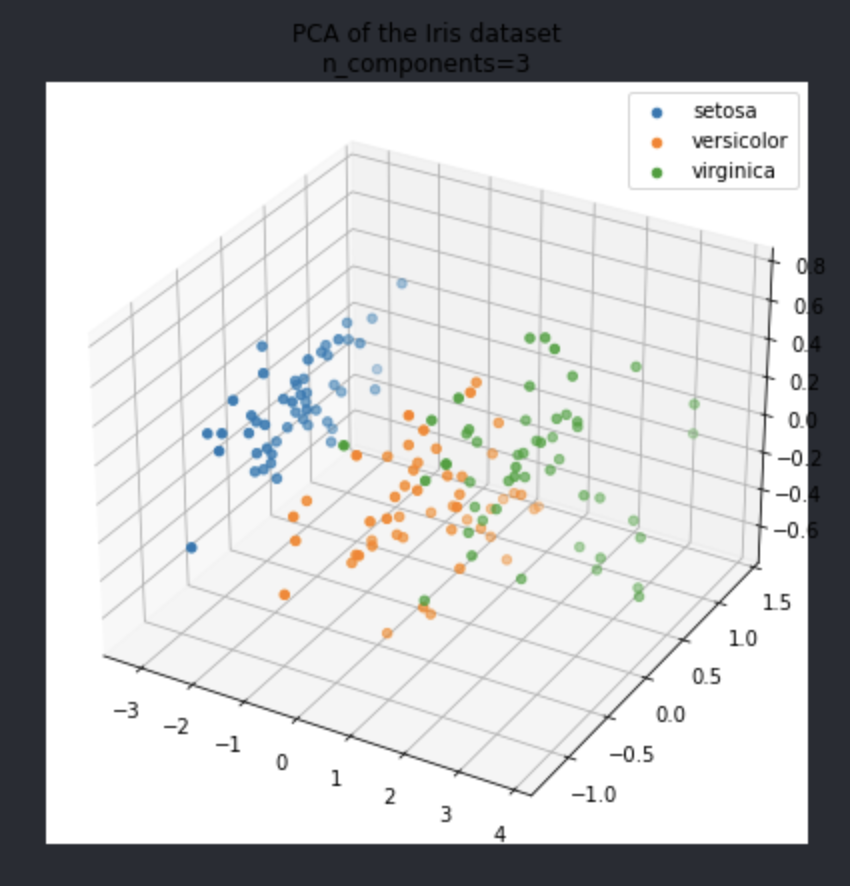
\includegraphics[width=\linewidth]{figures/pca.png}
    \caption{PCA Scatterplot}
    \label{fig:boat1}
  \end{figure}

\subsubsection{Data Pre-processing}

We performed a series of transformations to ensure that the data is properly prepared
for the neural network training. These transformations include:

\textbf{Scaling}: To avoid a scenario where features with larger values dominate the objective function, we scale the data to
    have zero mean and unit variance.
    
\textbf{One-hot encoding}: We convert categorical features into binary features through one-hot encoding. This transformation
    ensures that the model does not interpret categorical features as ordinal, which could lead to inaccurate classifications.
    
\textbf{Train-test split}: To evaluate the model's performance on unseen data, we divide the dataset into a training set and a
    test set. The training set is utilized for training the model, while the test set serves as a benchmark for assessing the
    model's generalization capabilities.

By applying these transformations to the iris datasey, we can effectively preprocess the data, enabling the neural
network to learn the underlying patterns and relationships more efficiently. This, in turn, will lead to more accurate and
reliable classification results.

\subsection{Neural Network Design}

\subsubsection{Topology and Architecture}

Our artificial neural network (ANN) is intricately designed to handle the task at hand. The input layer of our network is composed of four nodes, each corresponding to the four distinct attributes found within the Iris dataset. These attributes are sepal length, sepal width, petal length, and petal width. This layer serves as the gateway, allowing the data to flow into the network for further processing.

In a quest to find the optimal network architecture, we conducted multiple experiments. Specifically, we tested three different structures with varying hidden layer sizes and node configurations. These experiments aimed to understand the impact of the number of layers and nodes on the network's performance.

The output layer, the final stage of the network, is made up of three nodes. These nodes represent the three Iris species that our network aims to classify, namely, Iris Setosa, Iris Versicolour, and Iris Virginica.

By increasing the number of hidden layers and nodes within each layer, the network can learn more complex representations of the data. This, in turn, can significantly improve its ability to make accurate classifications. 

To enhance the learning within our network, we opted for the Rectified Linear Unit (RELU) as our activation function. This function is known for its higher threshold for activation, which means that it requires stronger evidence before firing a neuron. This characteristic can aid our network in learning more meaningful and sparser representations of the data, which is especially beneficial for the classification task at hand.

\subsubsection{Training Algorithm (Backpropagation)}

\subsection{Training and Testing}

We trained our deep neural network using the backpropagation algorithm, a key method in optimizing network weights and a gradient descent variant. This algorithm aims to minimize output layer error by adjusting hidden layer weights.

Training starts with a forward pass through the network, generating an initial prediction. The difference between this prediction and the actual value is calculated as an error via a loss function. Next, a backward pass computes the error derivative with respect to each weight, quantifying each weight's contribution to total error. Weights are updated to minimize error, and this process repeats until network performance plateaus or overfits.

We combined backpropagation with the stochastic gradient descent (SGD) optimization algorithm, efficient for large datasets, setting 'MaxEpochs' to 500 and 'InitialLearnRate' to 0.25. This combination was crucial for effective training and achieving performance on the Iris dataset, requiring careful balance of the learning rate and epochs.

Our architecture also included dropout layers and batch normalization, which contributed to effective learning, preventing overfitting, and ensuring the model generalized well to unseen data.

\subsubsection{Cross-validation}

To prevent overfitting and ensure our model generalises well, we used K-fold cross-validation, a robust statistical technique that assesses the model's performance on an independent dataset. We applied stratified 3-fold cross-validation on the Iris dataset, ensuring each fold represents the whole dataset's class label proportions, beneficial for imbalanced datasets.

This method involves dividing the dataset into 'K' subsets or 'folds', training on K-1 folds and validating on the held-out fold. Repeating this K times, each with a different validation fold, provides a reliable performance estimate on unseen data.

This method leverages the entire dataset for training and validation, advantageous for small datasets like ours. It gives insight into model performance across different data subsets, reducing overfitting likelihood and providing a reliable performance evaluation.

We used MATLAB's cvpartition function for efficient, unbiased data partitioning into training and validation sets, maximizing our data usage for model training while ensuring robust evaluation.

Correlation matrixes were generated an compared to ensure that the data was being split evenly and that the model was not overfitting.

\begin{figure}
    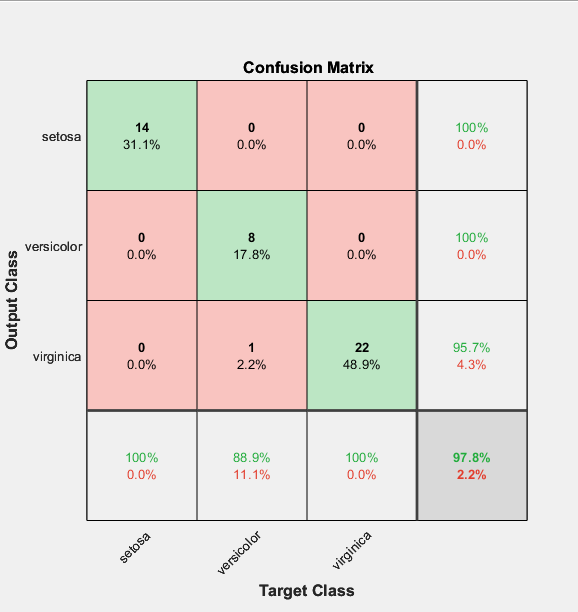
\includegraphics[width=\linewidth]{figures/Cm.png}
    \caption{Confusion Matrix}
    \label{fig:boat1}
  \end{figure}

\subsection{Results and Post-Processing}

The neural network works well, a series of confusion matrixes were generated after running for the designated number of epochs. They show that the neurual netowkr is predicting the flours accuratly but not too accuratly that it is overfitting. 

  \begin{figure}
    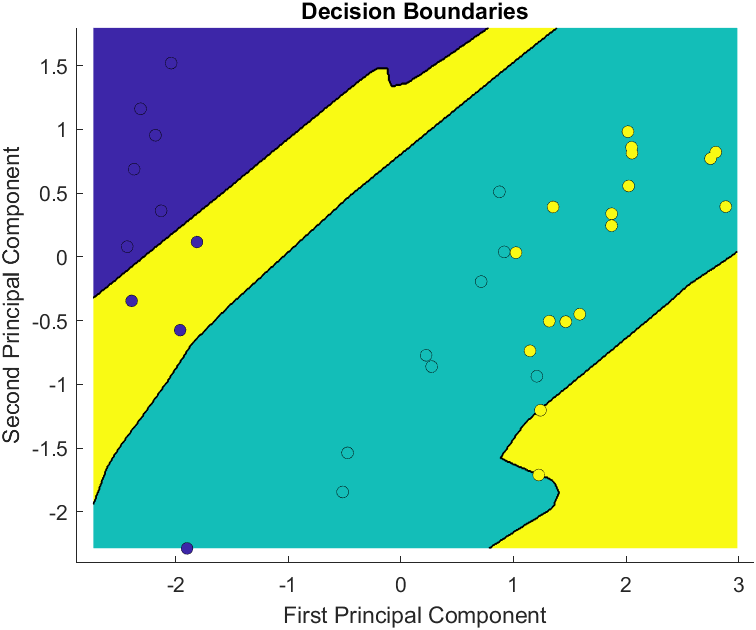
\includegraphics[width=\linewidth]{figures/DB.png}
    \caption{Decision Boundary}
    \label{fig:boat1}
  \end{figure}

  \begin{figure}
    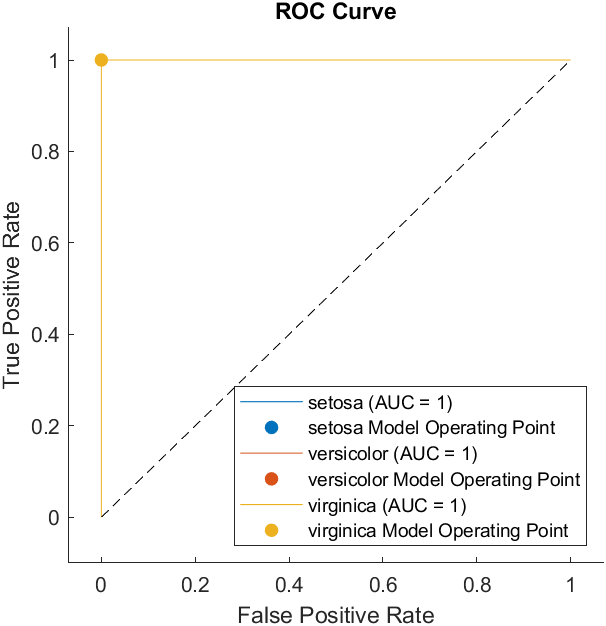
\includegraphics[width=\linewidth]{figures/roc.png}
    \caption{Decision Boundary}
    \label{fig:boat1}
  \end{figure}

\section{Part II: Genetic Algorithms for Global Optimization Problem}

\subsection{Function Selection and Analysis}

For the genetic algorithm section of our study, we've selected the Shubert function. This function, often used in optimization challenges, is characterized
by its complexity, featuring multiple local minima and maxima. This makes it an ideal choice for examining the robustness of genetic algorithms.

The Shubert function tests the algorithm's ability to navigate a landscape filled with local minima to find the global minimum. As the genetic algorithm
uses mechanisms inspired by natural evolution, it's well-suited for exploring a vast solution space.

Following this introduction, we'll provide details on the genetic algorithm's implementation, our chosen parameters, and the results of applying it to the
Shubert function, demonstrating its effectiveness in managing complex optimization problems.

\subsection{Genetic Algorithm Design}

The genetic algorithm (GA) design for this study is tailored towards optimizing the SHUBERT function, a complex and non-linear optimization problem known for its multiple local minima.

The SHUBERT function we used is a multivariate function defined as follows:

\begin{figure}
    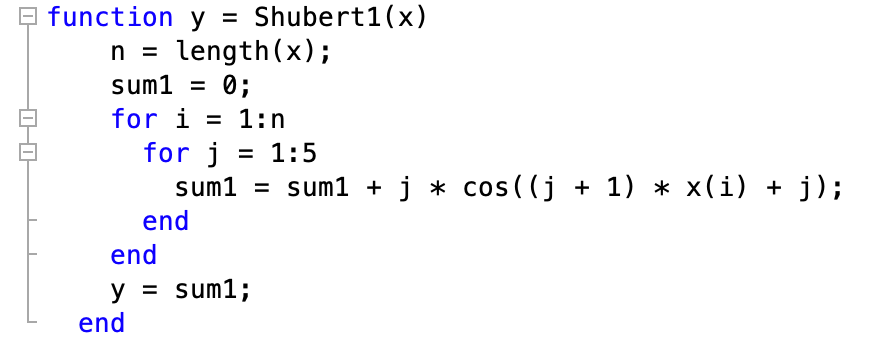
\includegraphics[width=\linewidth]{figures/shubertdes.png}
    \caption{Shubert Function Design}
    \label{fig:boat1}
  \end{figure}

In our study, we utilized a Genetic Algorithm (GA) for optimizing the SHUBERT function, a notoriously complex problem due to its multivariate and non-linear nature. The GA parameters were set with a population size of 400, promoting diversity and providing a broad search space.

The 'mutationadaptfeasible' and 'crossoverscattered' functions were chosen as mutation and crossover operations, respectively. The former adaptively scales the mutation based on previous success, while the latter randomly combines parent genes to produce offspring. 

We ensured the best two individuals from each generation (elite count of 2) were passed into the next, preserving high-quality solutions. A stochastic selection function 'selectionstochunif' was used to maintain a uniform distribution of sampling across the population, enhancing diversity.

The SHUBERT function optimization involved two variables, each ranging between -10 and 10. The GA was executed with these constraints, and the SHUBERT function served as the objective function. 


\subsubsection{Representation of Initial Population}

\begin{figure}
    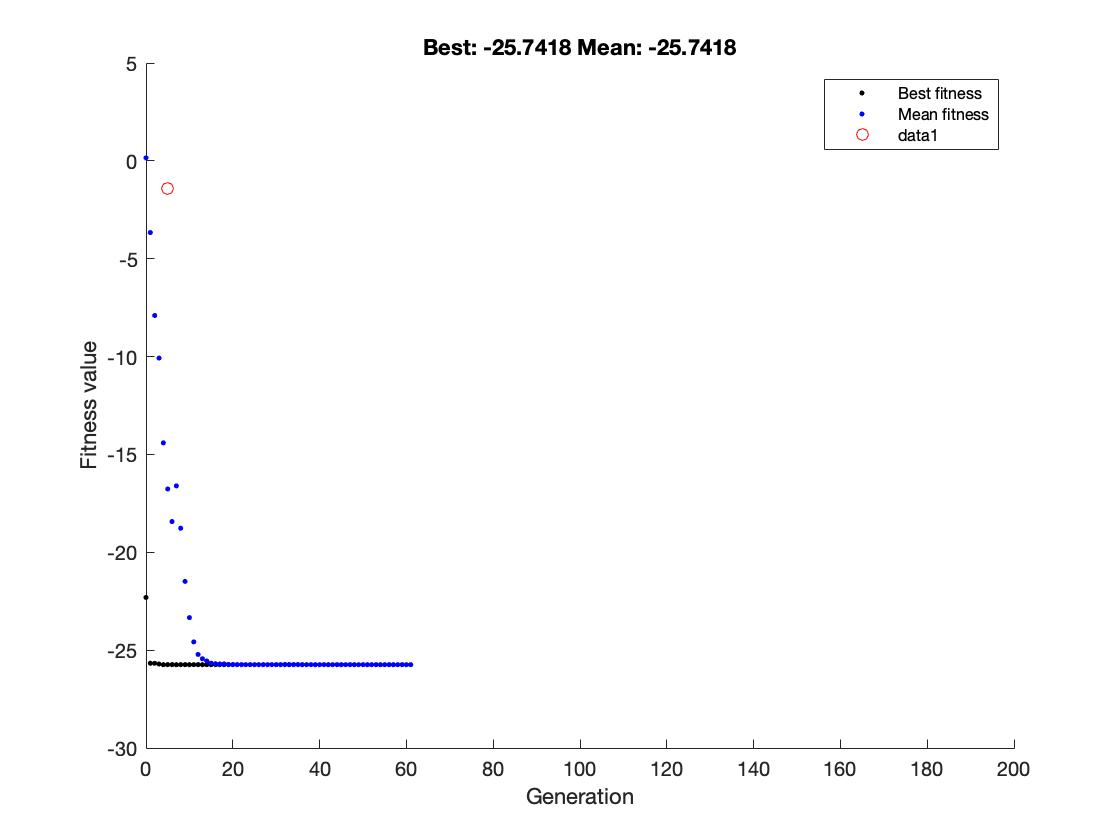
\includegraphics[width=\linewidth]{figures/shubert.jpg}
    \caption{Shubert Function}
    \label{fig:boat1}
  \end{figure}

\subsubsection{Fitness Function}

\subsubsection{Selection Method}

\subsubsection{Reproductive Operators}

\subsubsection{Stopping Criteria}

\subsubsection{Parameters and Constraints}
\subsection{GA Analysis of the Run}


\subsection{Results and Discussion}

\subsubsection{Premature Convergence}

\subsubsection{Maintaining Selection Pressure}

\subsubsection{Balancing Exploration and Exploitation}

\section{Conclusion}

\section*{References}


\bibliography{bib/IEEEabrv, bib/mybib}
\bibliographystyle{inc/IEEEtranS}


\end{document}